\documentclass[aspectratio=169]{beamer}

% ---------------------------------------------------
% PACKAGES & THEME SETUP
% ---------------------------------------------------
\usetheme{Madrid}

% Top section navigation bar
\useoutertheme[subsection=false]{miniframes}

% Define ISEG Red 
\definecolor{isegred}{RGB}{190, 15, 20}

% Apply the custom red color to the entire Beamer structure
\usecolortheme[named=isegred]{structure}

\usepackage{graphicx}
\usepackage{booktabs}
\usepackage{amsmath}
\usepackage{listings}
\usepackage{xcolor}

% ---------------------------------------------------
% PYTHON CODE STYLING (listings package)
% ---------------------------------------------------
\definecolor{codegreen}{rgb}{0,0.6,0}
\definecolor{codegray}{rgb}{0.5,0.5,0.5}
\definecolor{codepurple}{rgb}{0.58,0,0.82}
\definecolor{backcolour}{rgb}{0.95,0.95,0.92}

\lstdefinestyle{mystyle}{
    backgroundcolor=\color{backcolour},   
    commentstyle=\color{codegreen},
    keywordstyle=\color{isegred},    % Changed keywords to match the red theme!
    numberstyle=\tiny\color{codegray},
    stringstyle=\color{codepurple},
    basicstyle=\ttfamily\scriptsize, 
    breakatwhitespace=false,         
    breaklines=true,                 
    captionpos=b,                    
    keepspaces=true,                 
    numbers=left,                    
    numbersep=5pt,                  
    showspaces=false,                
    showstringspaces=false,
    showtabs=false,                  
    tabsize=2
}
\lstset{style=mystyle}

% ---------------------------------------------------
% TITLE PAGE INFORMATION
% ---------------------------------------------------
% Note: Using commas in the [] brackets prevents Beamer footer crashes!
\title[Drivers of Renewable Energy]{Macro-Level Drivers of Renewable Energy Adoption}
\subtitle{A Blended Machine Learning and Econometrics Approach}
\author[Barzegar, Qian, Kaliwoda, Dedov]{Reza Barzegar \and Cheng Qian \and Paulina Kaliwoda \and Daniil Dedov}
\institute[ISEG]{
  PDS - Programming for Data Science \\
  ISEG, Universidade de Lisboa
}
\date{April 19th, 2026}

% ---------------------------------------------------
% DOCUMENT BEGINS
% ---------------------------------------------------
\begin{document}

% Slide 1: Title Slide
\begin{frame}
  \titlepage
\end{frame}

% Slide 2: Agenda
\begin{frame}{Agenda}
  \tableofcontents
\end{frame}

% ===================================================
\section{Introduction}
% ===================================================

\begin{frame}{The Research Question}
  \vspace{0.5cm}
  \begin{center}
      \Large \textit{"What are the key socioeconomic indicators that are driving the adoption rate of renewable energy consumption for a given country profile?"}
  \end{center}
  \vspace{0.8cm}
  
  \textbf{The Limitation in Current Literature:}
  \begin{itemize}
      \item Global climate policies often prescribe uniform solutions (e.g., carbon pricing) across highly disparate economies.
      \item Traditional pooled regressions fail to account for unobserved structural heterogeneity, assuming a developing nation transitions exactly like an advanced economy.
  \end{itemize}
\end{frame}

\begin{frame}{The Main Objectives}
  % Mimicking the 4-block layout from the Project Proposal
  \begin{columns}[T]
    \begin{column}{0.48\textwidth}
      \begin{block}{01 | Data Processing}
        Transforming uncompiled raw datasets into one balanced, mathematically sound panel data.
      \end{block}
      \vspace{0.3cm}
      \begin{block}{03 | Statistical Analysis}
        Analyzing the significance of all the different macroeconomic variables strictly per classification.
      \end{block}
    \end{column}
    
    \begin{column}{0.48\textwidth}
      \begin{block}{02 | Country Classification}
        Grouping countries into distinct developmental profiles based on baseline socioeconomic indicators.
      \end{block}
      \vspace{0.3cm}
      \begin{block}{04 | Effects Analysis}
        Understanding the magnitude of the effects (elasticities) from the significant indicators to inform policy.
      \end{block}
    \end{column}
  \end{columns}
\end{frame}

% ===================================================
\section{Methodology \& Data}
% ===================================================

\begin{frame}{POST-DS Framework \& Data Sources}
  \textbf{Analytical Framework:}
  \begin{itemize}
      \item The study follows the \textbf{POST-DS} (Process Organization and Scheduling electing Tools for Data Science) methodology to ensure actionable business deployment.
  \end{itemize}
  \vspace{0.3cm}
  
  \textbf{Primary Data Sources (2012 -- 2021):}
  \begin{enumerate}
      \item \textbf{World Bank Group:} Macroeconomic capacity (GDP) and infrastructural maturity (Electricity/Clean Cooking access).
      \item \textbf{Our World in Data \& IEA:} Granular energy mix metrics, fossil fuel reliance, and the dependent variable (Renewable Energy Share \%).
  \end{enumerate}
\end{frame}

\begin{frame}{Data Preparation Pipeline}
  \textbf{From Raw Data to Analysis-Ready Panel:}
  \begin{itemize}
      \item \textbf{Integration:} Merged 18,291 raw observations down to a highly curated, balanced panel of \textbf{2,600 country-year observations}.
      \item \textbf{Imputation:} Addressed missing developing-nation data via linear interpolation, forward-filling, and backward-filling.
      \item \textbf{Winsorization:} Capped extreme macroeconomic outliers at the 1st and 99th percentiles to prevent skewed regressions.
      \item \textbf{Mathematical Normalization:} Applied shifted natural logarithmic transformations to heavily right-skewed variables (e.g., GDP per capita, Land Area).
  \end{itemize}
\end{frame}

\begin{frame}{Exploratory Data Analysis: Descriptive Statistics}
  \textbf{Key Insight:} Massive heterogeneity across global economies.
  
  \begin{table}[]
      \centering
      \footnotesize % Forces the table to use a smaller, slide-appropriate font
      \begin{tabular}{l c c c c c}
      \toprule
      \textbf{Variable} & \textbf{Mean} & \textbf{Std. Dev.} & \textbf{Min} & \textbf{Median} & \textbf{Max} \\
      \midrule
      Renewables Share (\%) & 17.99 & 16.09 & 0.00 & 14.10 & 82.90 \\
      GDP per Capita (USD) & 12,537 & 88,530 & 492 & 64,181 & 816,291 \\
      Access to Clean Cooking (\%) & 92.78 & 16.37 & 14.50 & 100.00 & 100.00 \\
      Energy per Capita (kWh) & 44,587 & 41,889 & 1,903 & 32,542 & 245,295 \\
      Fossil Electricity (TWh) & 206.58 & 624.90 & 0.00 & 49.98 & 5,678 \\
      \bottomrule
      \end{tabular}
  \end{table}
  \vspace{-0.2cm} % Pulls the footnote slightly closer to the table
  {\tiny \textit{*Note: Table displays a curated subset of 5 key variables for presentation visibility. The full analysis panel contains 18 variables.}}\par
  
  \vspace{0.2cm}
  \begin{itemize}
      \small % Makes the bullet points slightly smaller to ensure they fit
      \item \textbf{Skewness:} GDP and Energy exhibit extreme right-skewness (justifying the log-transformations).
      \item \textbf{Polarity:} Infrastructure access median is $100\%$, but minimums drop below $15\%$, justifying our regime-clustering approach.
  \end{itemize}
\end{frame}

\begin{frame}{Exploratory Data Analysis: Structural Multicollinearity}
  \begin{columns}[c]
    \begin{column}{0.55\textwidth}
      \textbf{The Multicollinearity Problem:}
      \begin{itemize}
          \item Initial variables exhibited severe cross-correlation (e.g., Absolute $\text{CO}_2$ vs. Total Fossil Fuel Generation).
          \item \textbf{Solution:} Applied a strict Pearson correlation threshold of $\rho > 0.80$.
          \item Highly collinear variables were systematically dropped to ensure matrix stability in the final fractional panel models.
      \end{itemize}
    \end{column}
    \begin{column}{0.45\textwidth}
      \centering
      % Ensure 'reduced_correlation_heatmap.png' is uploaded to your LaTeX project!
      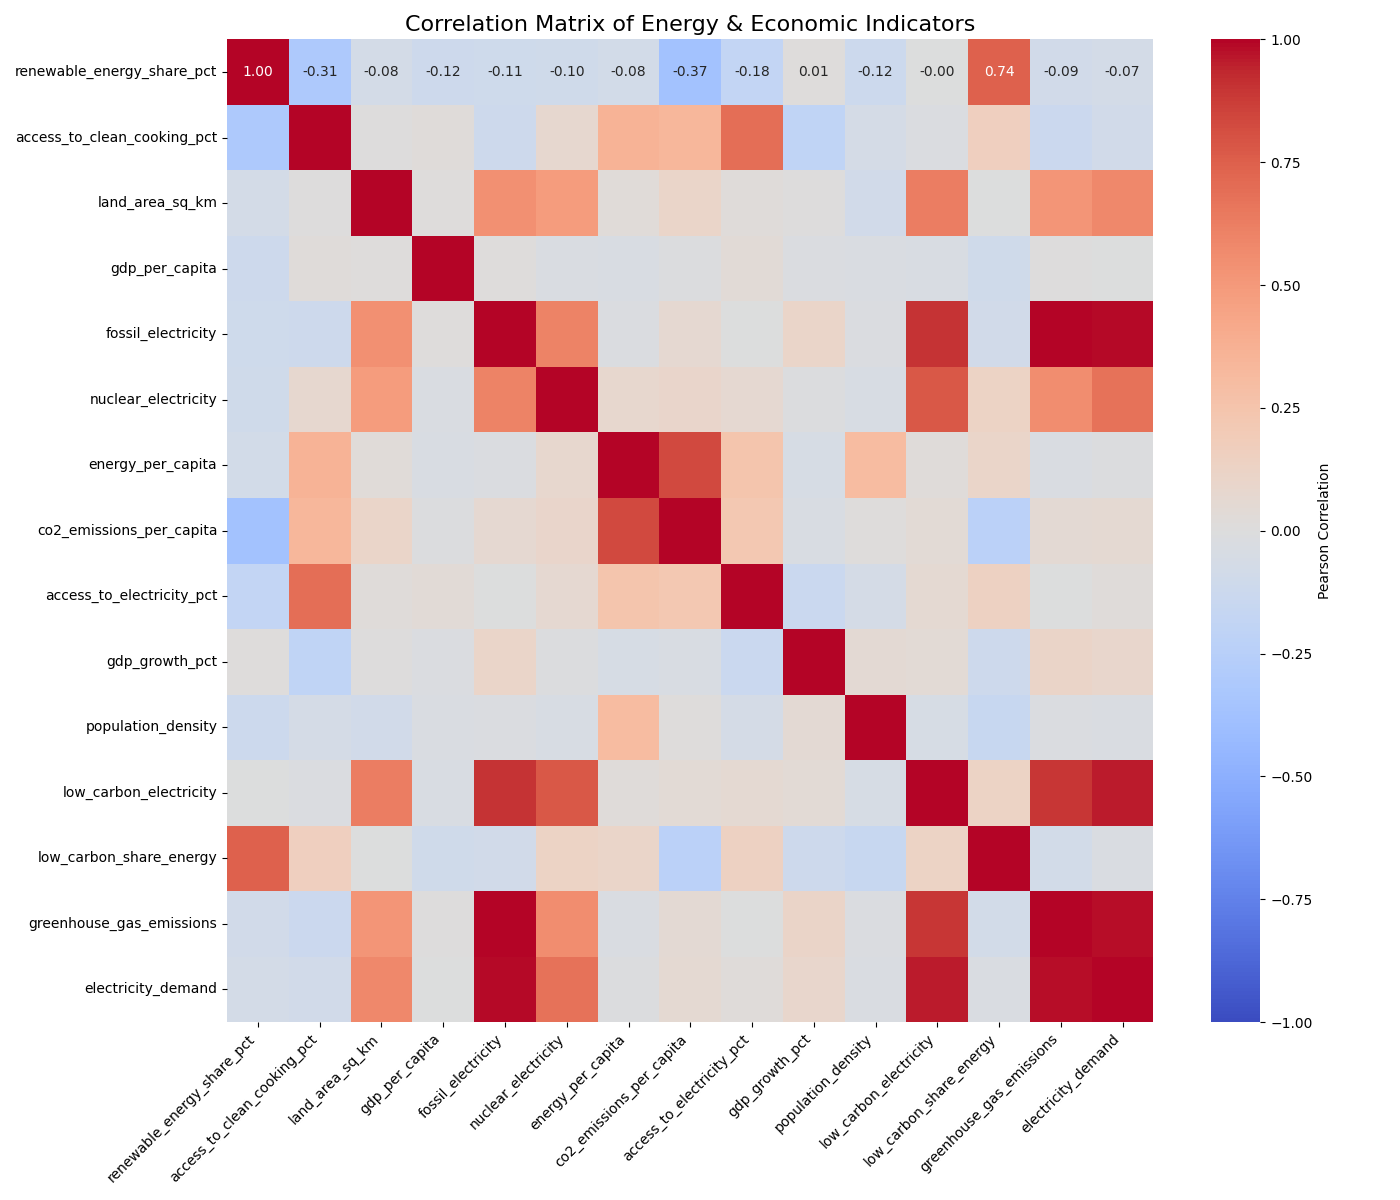
\includegraphics[width=\textwidth,keepaspectratio]{Image/correlation_heatmap.png}
    \end{column}
  \end{columns}
\end{frame}

% ===================================================
\section{I: Unsupervised Learning}
% ===================================================

\begin{frame}{1. Pre-FA Variable Selection}
  \textbf{Strategic Variable Splitting to Prevent Endogeneity}
  \vspace{0.2cm}
  
  For the Factor Analysis and clustering phase, the dataset was strictly restricted to six foundational macroeconomic and infrastructural traits.
  We excluded specific energy policy levers like Nuclear or Fossil generation so regimes are defined purely by baseline developmental maturity, rather than the specific energy generation choices we intend to evaluate later.
  
  \vspace{0.3cm}
  \textbf{The 6 Structural Variables Selected for FA:}
  \begin{enumerate}
      \item Access to Electricity (\%)
      \item Access to Clean Cooking (\%)
      \item GDP per Capita (USD)
      \item GDP Growth (\%)
      \item Energy per Capita (kWh)
      \item Baseline Low-Carbon Share of Energy (\%)
  \end{enumerate}
\end{frame}

\begin{frame}{2. OOP Architecture: \texttt{FactorAnalysisPrep} Class}
  \footnotesize 
  \textbf{Objective:} To cleanly isolate and mathematically normalize the 6 baseline variables prior to any machine learning applications.
  \vspace{0.1cm}

  \begin{description}
      \item[\texttt{handle\_outliers()}:] \hfill \\
      \textbf{Purpose:} Caps extreme values at the 1st and 99th percentiles. \\
      \textbf{Reasoning:} Prevents K-Means centroids and Factor variances from being disproportionately skewed by a single massive global economy.
      
      \item[\texttt{handle\_skewed\_distributions()}:] \hfill \\
      \textbf{Purpose:} Applies a \texttt{log1p} transformation to variables with high skewness, $>$1.5. \\
      \textbf{Reasoning:} Normalizes heavily right-skewed data to satisfy the distributional assumptions of variance-based algorithms.
      
      \item[\texttt{standardize\_data()}:] \hfill \\
      \textbf{Purpose:} Scales data to Mean = 0 and Standard Deviation = 1. \\
      \textbf{Reasoning:} Standardizing prevents variables with large raw numbers from dominating the clustering distance metrics.

      \item[\texttt{run\_tests()}:] \hfill \\
      \textbf{Purpose:} Executes VIF, Bartlett's and KMO tests. \\
      \textbf{Reasoning:} Confirm the variables share adequate common variance before proceeding.
  \end{description}
\end{frame}

\begin{frame}{3. OOP Architecture: \texttt{CountryProfiler} Class}
  \footnotesize 
  \textbf{Objective:} To execute the dimensionality reduction and clustering pipeline while dynamically determining the optimal parameters.
  \vspace{0.1cm}

  \begin{description}
      \item[\texttt{perform\_factor\_analysis()}:] \hfill \\
      \textbf{Purpose:} Uses the Kaiser Criterion, Eigenvalues $>$ 1, to determine the optimal number of factors, then extracts them using Varimax rotation. \\
      \textbf{Reasoning:} Reduces the 6 correlated baseline metrics down to unobserved, orthogonal dimensions to completely eliminate multicollinearity.

      \item[\texttt{determine\_optimal\_clusters()}:] \hfill \\
      \textbf{Purpose:} Computes K-Means for $K=2$ to $K=8$, evaluating the Elbow Method and the Silhouette Score. \\
      \textbf{Reasoning:} Empirically finds the best number of regimes by maximizing intra-cluster cohesion and inter-cluster separation, eliminating human bias.

      \item[\texttt{fit\_clusters()}:] \hfill \\
      \textbf{Purpose:} Fits K-Means on the Factor Scores and assigns profile labels to the original dataframe. \\
      \textbf{Reasoning:} Successfully groups nations into distinct developmental regimes for the subsequent econometric sample-splitting.
  \end{description}
\end{frame}

\begin{frame}{4. Final Output: Factor Loadings \& Latent Dimensions}
  \textbf{Kaiser Criterion Result:} 3 Optimal Latent Factors extracted (Eigenvalues $> 1$).
  \vspace{0.1cm}
  
  \begin{table}[]
      \centering
      \footnotesize
      \begin{tabular}{l c c c}
      \toprule
      \textbf{Structural Variable} & \textbf{Factor 1} & \textbf{Factor 2} & \textbf{Factor 3} \\
      \midrule
      Access to Clean Cooking (\%) & \textbf{0.93} & 0.06 & -0.14 \\
      Access to Electricity (\%) & \textbf{0.74} & 0.09 & 0.01 \\
      Energy per Capita & \textbf{0.70} & -0.11 & -0.05 \\
      Low-Carbon Share of Energy & 0.02 & \textbf{1.00} & -0.02 \\
      GDP per Capita & -0.02 & 0.02 & \textbf{0.70} \\
      GDP Growth (\%) & -0.20 & -0.10 & \textbf{0.17} \\
      \bottomrule
      \end{tabular}
  \end{table}
  \vspace{0.1cm}
  
  \textbf{Interpretation of the Latent Dimensions:}
  \begin{itemize}
      \small
      \item \textbf{Factor 1 (Infrastructure \& Consumption):} Captures physical grid maturity and total domestic energy demand.
      \item \textbf{Factor 2 (Energy Mix):} Strictly isolates the baseline green energy profile.
      \item \textbf{Factor 3 (Economic Wealth \& Growth):} Captures macroeconomic capacity and the rate of industrial expansion.
  \end{itemize}
\end{frame}

\begin{frame}{5. Final Output: The Identified Regimes}
  \begin{columns}[c]
    \begin{column}{0.45\textwidth}
      \centering
      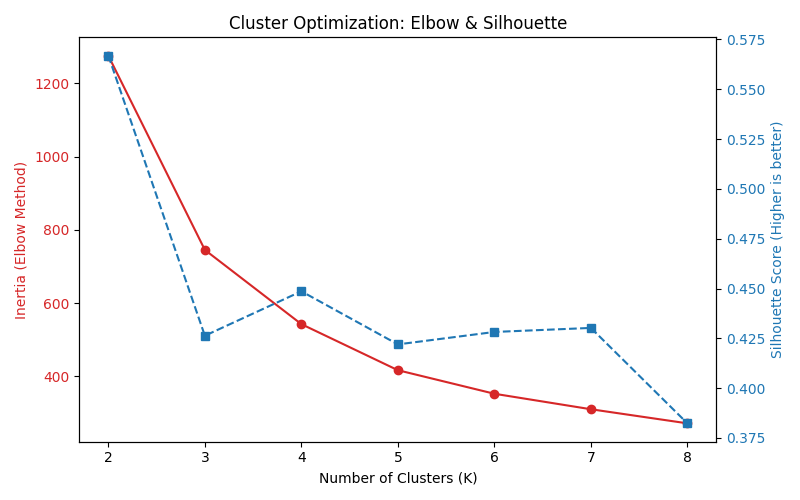
\includegraphics[width=\textwidth,keepaspectratio]{Image/Cluster_Optimization.png}
      \vspace{0.2cm}
      {\scriptsize \textit{Global Maximum Silhouette Score at K=2}}
    \end{column}
    
    \begin{column}{0.55\textwidth}
      \textbf{Cluster 0: Developed Regime}
      \begin{itemize}
          \item \textbf{Infrastructure:} 100\% Access.
          \item \textbf{Consumption:} Massive (34,152 kWh/capita).
          \item \textbf{Growth:} Slower, stable GDP growth.
      \end{itemize}
      \vspace{0.3cm}
      
      \textbf{Cluster 1: Developing Regime}
      \begin{itemize}
          \item \textbf{Infrastructure:} Incomplete (41\% Clean Cooking, 92\% Electricity).
          \item \textbf{Consumption:} Lower (4,220 kWh/capita).
          \item \textbf{Growth:} Rapid industrial expansion (6.34\%).
      \end{itemize}
    \end{column}
  \end{columns}
\end{frame}

% ===================================================
\section{II: Time Series Analysis}
% ===================================================

\begin{frame}{1. Theoretical Background: Temporal Dynamics}
  \textbf{Why analyze time series before panel econometrics?}
  \vspace{0.2cm}
  
  Energy infrastructure possesses massive physical inertia, making the transition rate highly path-dependent. 
  Before executing our fractional panel models, we must evaluate the dependent variable (Renewable Energy Share) over the 2012--2021 decade to test for stationarity and temporal stickiness.
  \vspace{0.3cm}
  
  \textbf{Key Objectives:}
  \begin{itemize}
      \item \textbf{Prevent Spurious Regressions:} Identify if the data is trending endlessly (non-stationary), which violates standard regression assumptions and produces artificially low p-values.
      \item \textbf{Measure Inertia:} Quantify how much last year's grid dictates this year's energy mix.
      \item \textbf{Assess Global Convergence:} Determine if the gap between leading and lagging nations is shrinking, or actively widening over time.
  \end{itemize}
\end{frame}

\begin{frame}{2. OOP Architecture: \texttt{TimeSeriesAnalyzer} Class}
  \footnotesize 
  \textbf{Objective:} Programmatically analyze the temporal trajectory, stationarity, and global convergence of renewable energy adoption.
  \vspace{0.1cm}

  \begin{description}
      \item[\texttt{test\_stationarity()}:] \hfill \\
      \textbf{Purpose:} Executes the Augmented Dickey-Fuller (ADF) test to check for a unit root. \\
      \textbf{Reasoning:} If the series is non-stationary, it mandates the inclusion of Time Fixed Effects in the final econometric models to prevent spurious, invalid results.

      \item[\texttt{plot\_autocorrelation()}:] \hfill \\
      \textbf{Purpose:} Generates ACF and PACF plots for the global time series. \\
      \textbf{Reasoning:} Measures transition inertia. Extreme autocorrelation at Lag 1 confirms that a nation's energy mix is heavily anchored by its pre-existing physical infrastructure.

      \item[\texttt{analyze\_convergence()}:] \hfill \\
      \textbf{Purpose:} Calculates the standard deviation of renewable adoption across all countries for each year. \\
      \textbf{Reasoning:} Tracks whether global climate policies are successfully equalizing transition rates (convergence) or if they are polarizing them (divergence).
  \end{description}
\end{frame}

\begin{frame}{3. Final Output: Macro Trend Analysis}
  \begin{columns}[c]
    \begin{column}{0.55\textwidth}
      \centering
      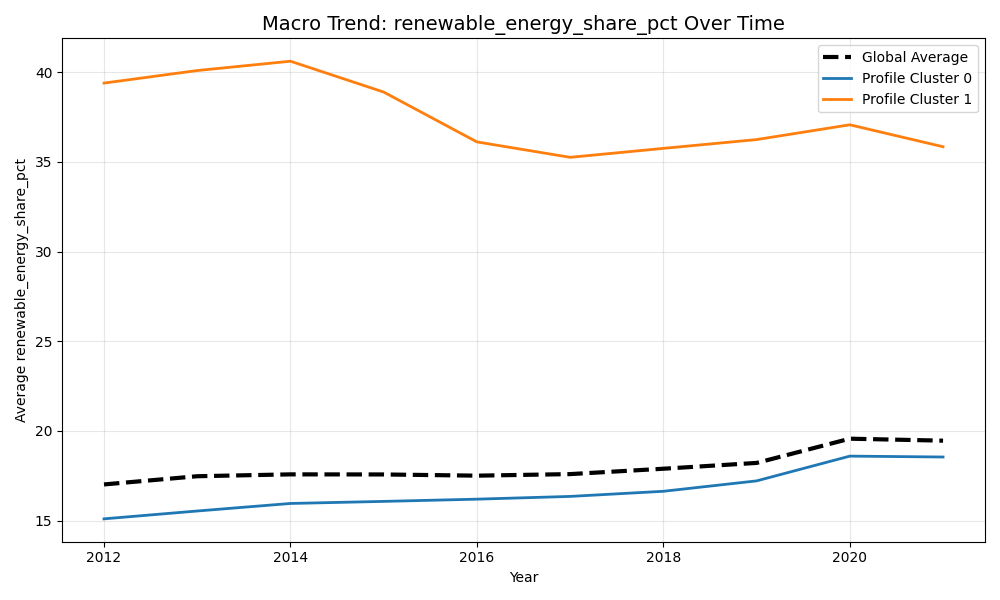
\includegraphics[width=\textwidth,keepaspectratio]{Image/TSA_Macro_Trends.png}
    \end{column}
    
    \begin{column}{0.45\textwidth}
      \textbf{Global Trajectory}
      \begin{itemize}
          \small
          \item Both developmental regimes exhibit clear upward trajectories, particularly accelerating post-2015, reflecting the momentum of the Paris Agreement.
          \item \textbf{Structural Gap:} Despite mutual growth, a massive absolute gap persists between the baseline of the Developed (Cluster 0) and Developing (Cluster 1) regimes.
      \end{itemize}
    \end{column}
  \end{columns}
\end{frame}

\begin{frame}{4. Final Output: Stationarity \& Path Dependency}
  \begin{columns}[c]
    \begin{column}{0.55\textwidth}
      \centering
      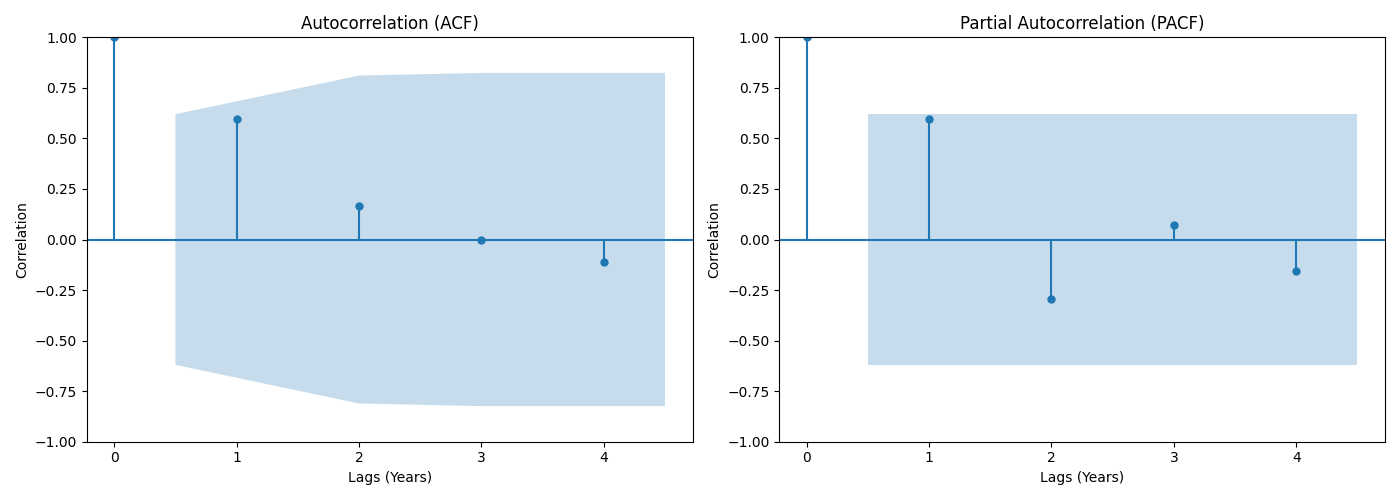
\includegraphics[width=\textwidth,keepaspectratio]{Image/TSA_Autocorrelation.png}
    \end{column}
    
    \begin{column}{0.45\textwidth}
      \textbf{ADF Stationarity Test}
      \begin{itemize}
          \footnotesize
          \item \textbf{Statistic:} 0.4416 | \textbf{P-Value:} 0.9830
          \item \textbf{Result:} Non-Stationary.
          \item \textbf{Impact:} Time-Fixed effects are strictly required for our fractional models.
      \end{itemize}
      \vspace{0.3cm}
      
      \textbf{Autocorrelation (Inertia)}
      \begin{itemize}
          \footnotesize
          \item Severe autocorrelation observed at Lag 1 (seen in the ACF plot).
          \item \textbf{Result:} High \textbf{path-dependency}. A nation's ability to transition is heavily anchored by the physical inertia of its existing legacy grid.
      \end{itemize}
    \end{column}
  \end{columns}
\end{frame}

\begin{frame}{5. Final Output: Policy Convergence Analysis}
  \begin{columns}[c]
    \begin{column}{0.55\textwidth}
      \centering
      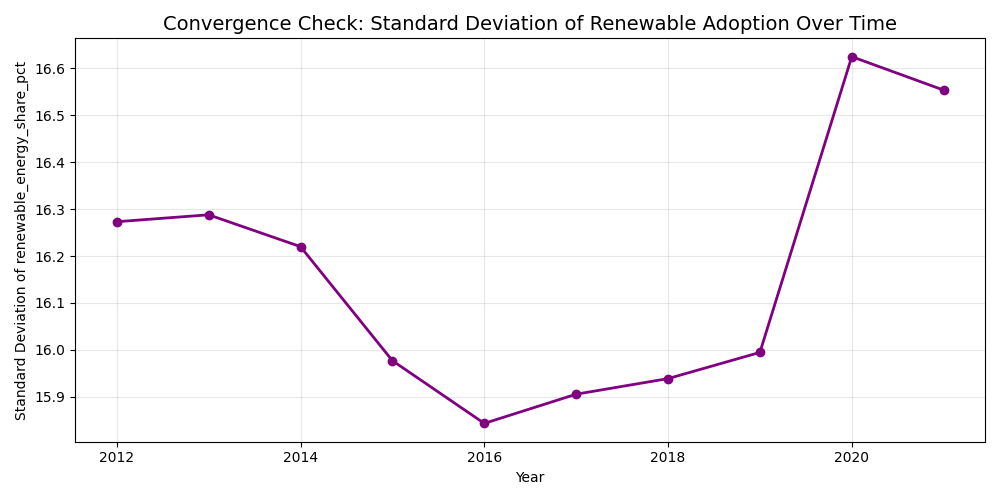
\includegraphics[width=\textwidth,keepaspectratio]{Image/TSA_Convergence.png}
    \end{column}
    
    \begin{column}{0.45\textwidth}
      \textbf{Tracking the Global Gap}
      \begin{itemize}
          \small
          \item The standard deviation of renewable adoption across all countries increased steadily from 2016 to 2021.
          \item \textbf{Conclusion:} \textbf{Global Divergence} is occurring. 
          \item \textbf{Impact:} Rather than equalizing, the statistical gap between green leaders and fossil-reliant nations is actively widening, highlighting the failure of uniform global policies.
      \end{itemize}
    \end{column}
  \end{columns}
\end{frame}

% ===================================================
\section{III: Econometrics Modeling}
% ===================================================

\begin{frame}{1. Theoretical Background: The Bounded Data Problem}
  \textbf{Why traditional Ordinary Least Squares (OLS) fails here:}
  \vspace{0.2cm}
  
  Our dependent variable (Renewable Energy Share) is a percentage, strictly bounded between 0 and 100. If we use a standard linear OLS regression, the model is mathematically misspecified and can predict impossible values (e.g., -15\% or 120\% renewable energy). 
  
  \vspace{0.3cm}
  \textbf{The Fractional Solution:}
  To respect the physical boundaries of the data, we must deploy non-linear econometric techniques. We utilize two distinct approaches:
  \begin{itemize}
      \item \textbf{Papke \& Wooldridge (2008):} A Correlated Random Effects (CRE) Fractional Probit model that naturally maps predictions to a $[0, 1]$ curve.
      \item \textbf{Ramalho \& Ramalho (2017):} A Log-Odds transformation that mathematically stretches the bounded data to $(-\infty, +\infty)$, allowing us to safely use standard Panel Fixed Effects.
  \end{itemize}
\end{frame}

\begin{frame}{2. OOP Architecture: \texttt{AdvancedDataProcessing} Class}
  \footnotesize 
  \textbf{Objective:} To reintroduce the broader set of policy variables and systematically filter multicollinearity before regression matrix inversion.
  \vspace{0.1cm}

  \begin{description}
      \item[\textbf{Difference from \texttt{FactorAnalysisPrep}:}] \hfill \\
      While the FA prep strictly isolated 6 baseline variables, \textit{this} class dynamically ingests all 14 independent variables (including policy levers like Nuclear and Fossil generation) to prep them for econometric testing.
      
      \item[\texttt{drop\_highly\_correlated(threshold=0.80)}:] \hfill \\
      \textbf{Purpose:} Computes a Pearson correlation matrix and programmatically drops variables that exceed a $0.80$ threshold. \\
      \textbf{Reasoning:} Fixed Effects panel models require matrix inversion. Severe collinearity (e.g., Total $\text{CO}_2$ vs. Fossil Generation) causes the inversion to fail. This function dynamically saved our subset down to 11 mathematically stable predictors.
  \end{description}
\end{frame}

\begin{frame}{3. OOP Architecture: \texttt{AdvancedPanelModeler} Class}
  \footnotesize 
  \textbf{Objective:} To execute regime-specific fractional models while controlling for unobserved country heterogeneity and time trends.
  \vspace{0.1cm}

  \begin{description}
      \item[\texttt{run\_pw2008\_cre\_fractional\_probit()}:] \hfill \\
      \textbf{Purpose:} Fits a Generalized Linear Model (GLM) with a Binomial family and Probit link. \\
      \textbf{Reasoning:} Standard non-linear models suffer from the "incidental parameters problem" when traditional fixed effects are introduced. We solved this using the Chamberlain-Mundlak device, calculating the country-level means (\texttt{X\_means}) to safely control for unobserved heterogeneity.

      \item[\texttt{run\_ramalho2017\_transformed\_fe()}:] \hfill \\
      \textbf{Purpose:} Applies a Log-Odds boundary adjustment, then runs \texttt{PanelOLS}. \\
      \textbf{Reasoning:} By stretching the data boundaries, we were able to explicitly invoke \texttt{time\_effects=True}. This directly addressed the Non-Stationary finding from our ADF Time Series test, ensuring our p-values were entirely robust against global time trends.
  \end{description}
\end{frame}

\begin{frame}{4. Final Output: Regime-Specific Drivers}
  \vspace{-0.2cm} % Pulls the content up closer to the header
  {\small \textbf{Key Insight:} Drivers of renewable energy depend entirely on the developmental regime.}
  
  \begin{table}[]
      \centering
      \scriptsize % Shrinks the table font slightly more
      \begin{tabular}{l c c | c c}
      \toprule
      & \multicolumn{2}{c|}{\textbf{Cluster 0: Developed}} & \multicolumn{2}{c}{\textbf{Cluster 1: Developing}} \\
      \textbf{Variable} & \textbf{PW2008} & \textbf{Ramalho} & \textbf{PW2008} & \textbf{Ramalho} \\
      \midrule
      GDP per Capita & $0.2300^{***}$ & $0.4567$ & $-0.2308$ & $-0.2808$ \\
      Clean Cooking (\%) & $-0.6915$ & $-0.8691^{***}$ & $0.6050$ & $1.0763$ \\
      Land Area & $0.5142$ & $3.2100$ & $6.5223$ & $8.2908^{***}$ \\
      Fossil Electricity & $-0.1825$ & $-0.2996^{***}$ & $-0.3385^{***}$ & $-0.4793$ \\
      \bottomrule
      \end{tabular}
  \end{table}
  \vspace{-0.2cm}
  {\tiny\textit{Significance: *** $p<0.01$. Standard errors clustered by country. Showing 4 focal variables.}}\par
  
  \vspace{0.1cm}
  \begin{itemize}
      \footnotesize
      \item \textbf{Wealth Divergence:} GDP drives renewables in advanced grids but hinders them in rapidly industrializing nations.
      \item \textbf{Infrastructure Catalyst:} Clean cooking access acts as a massive catalyst exclusively for the Developing regime.
      \item \textbf{Universal Barrier:} Entrenched Fossil Electricity holds a significantly negative drag across both regimes (Carbon Lock-in).
  \end{itemize}
\end{frame}

% ===================================================
\section{Results \& Discussion}
% ===================================================

\begin{frame}{1. Discussion: The Developed Regime (Cluster 0)}
  \textbf{The Reality of Advanced Economies:}
  \vspace{0.2cm}
  
  Our models (PW2008 \& Ramalho2017) reveal that for nations with fully mature infrastructure, the transition is primarily constrained by legacy systems rather than capital.
  
  \vspace{0.3cm}
  \begin{itemize}
      \item \textbf{The Wealth Effect:} GDP per Capita shows a strong positive correlation ($0.2300^{***}$). In advanced economies, excess capital is actively being deployed into green R\&D and grid modernization. Renewable energy acts as a luxury or "normal" good.
      \item \textbf{Carbon Lock-In:} Fossil Electricity demonstrates a significant negative coefficient ($-0.2996^{***}$). This empirically proves the "inertia" we found in our Time Series analysis: existing, highly profitable fossil fuel infrastructure actively crowds out green investment.
  \end{itemize}
\end{frame}

\begin{frame}{2. Discussion: The Developing Regime (Cluster 1)}
  \textbf{The Reality of Industrializing Economies:}
  \vspace{0.2cm}
  
  For Cluster 1, the transition is not about modernizing an old grid; it is about building the grid in the first place while simultaneously trying to grow the economy.
  
  \vspace{0.3cm}
  \begin{itemize}
      \item \textbf{The Growth Paradox:} Unlike advanced nations, GDP growth here is inherently tied to carbon-intensive industrialization. Economic expansion currently requires cheap, fast, and scalable energy (coal/gas), temporarily depressing the renewable share.
      \item \textbf{The Infrastructure Catalyst:} Access to Clean Cooking is a massive positive driver. Modernizing baseline human infrastructure acts as a gateway; once a population secures basic energy security, the nation can pivot toward integrating distributed renewables like solar.
      \item \textbf{Geographical Advantage:} Land Area has a massive coefficient ($8.2908^{***}$). Developing nations with vast territories have a unique advantage to leapfrog traditional grids by deploying decentralized, utility-scale solar and wind.
  \end{itemize}
\end{frame}

\begin{frame}{3. Answering the Research Question}
  \begin{center}
      \Large \textit{"What are the key socioeconomic indicators driving adoption for a given country profile?"}
  \end{center}
  \vspace{0.6cm}
  
  \textbf{The Verdict: One Size Does Not Fit All}
  \begin{table}[]
      \centering
      \small
      \begin{tabular}{p{4cm} p{5cm} p{5cm}}
      \toprule
      \textbf{Metric} & \textbf{Cluster 0 (Developed)} & \textbf{Cluster 1 (Developing)} \\
      \midrule
      \textbf{Primary Barrier} & Physical Fossil Inertia & Lack of Basic Infrastructure \\
      \textbf{Role of GDP} & Accelerates Renewables & Temporarily Hinders Renewables \\
      \textbf{Optimal Policy Focus} & Carbon Pricing \& Early Retirement of Fossil Plants & Subsidized Grid Expansion \& Clean Cooking Access \\
      \bottomrule
      \end{tabular}
  \end{table}
\end{frame}

% ===================================================
\section{Conclusion}
% ===================================================

\begin{frame}{1. Executive Conclusion}
  \textbf{Methodological \& Empirical Success:}
  \vspace{0.2cm}
  
  \begin{itemize}
      \item \textbf{Architectural Triumph:} We successfully deployed an end-to-end Object-Oriented pipeline. By strictly separating Unsupervised ML, to identify regimes, from Fractional Econometrics, to calculate effects, we completely eliminated human bias from the global classification.
      \item \textbf{The End of Uniformity:} The data unequivocally proves that global climate policy cannot be uniform. A blanket carbon tax might work for Cluster 0 (Developed), but it would actively punish Cluster 1 (Developing) where fossil fuels are currently a strict prerequisite for escaping poverty.
      \item \textbf{Global Divergence:} As proven by our Time Series Convergence analysis, the gap between the green leaders and the lagging nations is actively widening. 
  \end{itemize}
\end{frame}

\begin{frame}{2. Policy Deployment (Actionable Insights)}
  \textbf{How global institutions (e.g., World Bank, IMF) should use this model:}
  \vspace{0.3cm}
  
  \begin{description}
      \item[For Developed Nations (Cluster 0):] \hfill \\
      \textbf{Target:} Overcoming "Carbon Lock-in." \\
      \textbf{Action:} Policies must explicitly financially penalize legacy fossil grid maintenance to force the retirement of old plants, making room for the wealth-driven green transition.

      \vspace{0.2cm}
      \item[For Developing Nations (Cluster 1):] \hfill \\
      \textbf{Target:} Infrastructure as a Gateway. \\
      \textbf{Action:} International green funds should \textit{not} just subsidize solar panels; they must heavily subsidize foundational infrastructure (like Access to Clean Cooking and basic grid stability). Once baseline survival needs are met, renewable integration naturally follows.
  \end{description}
\end{frame}

\begin{frame}{3. Limitations \& Future Work}
  \begin{columns}[T]
    \begin{column}{0.48\textwidth}
      \textbf{Current Limitations}
      \begin{itemize}
          \small
          \item \textbf{Temporal Scope:} The strict 10-year panel (2012-2021) was necessary for data completeness but limits long-term historical trend analysis.
          \item \textbf{Omitted Variables:} The model does not account for political stability, institutional corruption, or geospatial solar/wind potential.
      \end{itemize}
    \end{column}
    
    \begin{column}{0.48\textwidth}
      \textbf{Future Research Avenues}
      \begin{itemize}
          \small
          \item \textbf{Predictive Forecasting:} Transitioning from explanatory econometrics to predictive Machine Learning (e.g., XGBoost, LSTM) to forecast 2030 adoption rates.
          \item \textbf{Dynamic Panel Models:} Implementing Arellano-Bond (GMM) estimators to mathematically solve the extreme Lag 1 autocorrelation found in our time series.
      \end{itemize}
    \end{column}
  \end{columns}
\end{frame}

\begin{frame}[c] % [c] vertically centers the content
  \begin{center}
      \Huge \textbf{Thank You.} \\[0.5cm]
      \Large \textit{Questions \& Discussion}
  \end{center}
\end{frame}

\end{document}